\documentclass[12pt]{jbook}
% shuron.sty の漢字コードに注意
\usepackage{fancyhd,shuron}
\usepackage{graphics}
\usepackage[dvipdfm]{graphicx}
\usepackage{epsfig}
\usepackage{tabularx}
\usepackage{chapterbib}
\usepackage{makeidx}
\usepackage{amssymb}
\usepackage{url}
\usepackage{slashbox}
\usepackage{mediabb}

\makeatletter
\def\thefootnote{\ifnum\c@footnote>\z@\leavevmode\lower.5ex%
    \hbox{$^{*\@arabic\c@footnote}$}\fi}
\makeatother

\makeindex

\input{jdummy.def}

\begin{document}
\setcounter{page}{0}
\thispagestyle{empty}

\noindent
\includegraphics[height=2.0cm]{img/Lissajous_UEC_logo.eps}\\
\begin{tabular}{c}
{\Large 平成25年度 卒業論文}				\\
\end{tabular}

\vspace{2.5cm}

\begin{center}
\LARGE \bf Twitterを用いた携帯端末における \\
個人認証の多要素化に関する研究 \\
%\vspace{4mm}
\end{center}

\vspace{1.5cm}

\LARGE
\begin{flushright}
電気通信大学 情報理工学部 総合情報学科\\
1010086 高浪 悟\\

\vspace{1.6zh}

{\def\arraystretch{0.6}
\begin{tabular}{rll@{}}
指導教官	& 高田 哲司& 准教授	\\
							\\
提出日	& \multicolumn{2}{c@{}}{平成26年1月31日}	\\
\end{tabular}
}
\end{flushright}
\normalsize
\newpage

\thispagestyle{empty}

\noindent
\begin{center}
\LARGE \bf 概要\\
\end{center}

\vspace{1.0cm} 
{\small
概要(アブストラクト)は章とせず、以下の内容を1ページに要領良くまとめる.

\begin{itemize}
\setlength{\itemsep}{-2mm}
\item 研究の背景(学術的、社会的)
\item 目的
\item 方法
\item 結論
\end{itemize}

あいうえお かきくけこ さしすせそ たちつてと
あいうえお かきくけこ さしすせそ たちつてと
あいうえお かきくけこ さしすせそ たちつてと
あいうえお かきくけこ さしすせそ たちつてと
あいうえお かきくけこ さしすせそ たちつてと
あいうえお かきくけこ さしすせそ たちつてと
あいうえお かきくけこ さしすせそ たちつてと
あいうえお かきくけこ さしすせそ たちつてと

なにぬねの はひふへほ まみむめも やいゆえよ
なにぬねの はひふへほ まみむめも やいゆえよ
なにぬねの はひふへほ まみむめも やいゆえよ
なにぬねの はひふへほ まみむめも やいゆえよ
なにぬねの はひふへほ まみむめも やいゆえよ
なにぬねの はひふへほ まみむめも やいゆえよ
なにぬねの はひふへほ まみむめも やいゆえよ
なにぬねの はひふへほ まみむめも やいゆえよ
なにぬねの はひふへほ まみむめも やいゆえよ
なにぬねの はひふへほ まみむめも やいゆえよ

わをん わをん わをん わをん わをん わをん わをん
わをん わをん わをん わをん わをん わをん わをん
わをん わをん わをん わをん わをん わをん わをん
わをん わをん わをん わをん わをん わをん わをん
わをん わをん わをん わをん わをん わをん わをん
わをん わをん わをん わをん わをん わをん わをん

な、研究を行った.
}
\normalsize
\newpage


\setcounter{page}{1}

% 目次
\tableofcontents
% 図目次
\listoffigures
% 表目次
\listoftables

% 論文本体
%序論背景と目的
\chapter{序論}\label{chap:introduction}
\section{背景}
通信網の高速化・大容量化,電子機器の小型化・高性能化などにより,Webサービスで可能なことが多くなった.
また,高性能な携帯端末の普及により,個人や決済にかかわる重要な情報を持ち歩くことが一般化しつつあり,必然的に個人認証を行う場面が増えてきている.
こういった場面における個人認証では,パスワードや,PIN\footnote{Personal Identification Number,暗証番号.本論文においてこれを用いた認証という場合には,特に指定がない限り4桁の数字を秘密情報としたものを想定する.}を用いた例をよく見かける.

特にパスワードを用いた認証では,安全性と記憶持続性・利便性に関してはトレードオフの関係が存在する.
例えば,辞書攻撃に強い安全なパスワードを用いようとする際には,意味のない文字列にすることが望ましい.
しかし,意味のない文字列というのは憶えることが難しく,ユーザがパスワードを他のサービスにおいても使い回してしまう可能性が高まり,どれか一つのサービスからパスワードが流出した際,かえって脆弱になってしまう恐れがある.
現在,こういった問題を防ぐものとして,多要素認証を自由意志で利用できるWebサービスが増加しつつある.
例えば,パスワードの入力が完了し,それが正しいものだと判断された後に,あらかじめ登録された電話番号にSMS\footnote{Short Message Service,電話番号を利用して短いメッセージを送受信できるサービス}を利用して乱数を送信し,その乱数をそのまま入力させるといった方式をとることができる.
これにより,覗き見,推測や総当り攻撃によってパスワードが漏洩した際の不正利用のリスクを減少させることができるというメリットがある.

また,SNS\footnote{Social Networking Service,社会的ネットワークをインターネット上で構築するサービス.}の形態を持つWebサービスが近年増えてきている.
これにより,コミュニケーションの道具やライフログとして自分自身の情報を公開することが多くのユーザ間で一般的になりつつある.
SNSにおいては,公開範囲をある程度任意に指定できるサービスが多いという特徴がある.

\section{研究目的}
現在行われている個人認証の多要素化は,セキュリティトークンやEメールを用いたものが一般的であり,それにより大きく認証の安全性を高めている.しかし,利便性という点においては,一度認証のための画面から目を逸らす必要がある,特別なハードウェアを持ち歩く必要があるなど,今後の普及に際して改善の余地があると考えられる.

本研究ではSNSの情報を用いた個人認証の提案が少ないことに着目し,応用可能な典型例として携帯端末に搭載することを想定したシステムを考案した.本研究における目的は,SNSの情報を用いて記憶持続性と利便性に考慮しつつ個人認証の安全性を向上させることである.

\newpage

\section{論文の構成}
本論文は以下の章により構成される.\\
\\
第 \ref{chap:introduction} 章 序論:ここでは,本研究を行うに至った背景と主たる目的に関する解説を行う.\\
第 \ref{chap:preparation} 章 個人認証の多要素化への流れ:ここでは,認証技術の現状や,近年普及した技術が個人認証へ及ぼすと考えられる影響について述べる.\\
第 \ref{chap:relatedwork} 章 関連研究/製品:この章では,前章で述べた内容に関連する,既存の製品や研究の取り組みを紹介する.\\
第 \ref{chap:system} 章 Twitter上の情報を用いた提案認証システム:ここでは,本研究で開発したシステムに関する原理と詳細説明を行う.\\
第 \ref{chap:experiment} 章 検証実験:この章では,本研究で開発したシステムを用いた実験についての内容と結果の説明を行う.\\
第 \ref{chap:discussion} 章 考察:ここでは,これまでの取り組みと得られた結果から,本研究の成果と各結果に対する考察,ならびに今後の課題について考察する.\\
第 \ref{chap:conclusion} 章 結論:ここで本研究について総括する.\\

\newpage


%関連研究
\chapter{個人認証の多要素化への流れ}\label{chap:preparation}

\section{既存の認証技術}
一般に認証手法は以下の3つに大別できる.
\begin{itemize}
\item 知識認証
\item 所有物認証
\item 生体認証
\end{itemize}
これらの詳細は,以降の小節で述べる.

\subsection{知識認証}\label{subsec:knowledge}
本人のみが記憶している情報を秘密情報として認証を行う手法.
主にキーボードやタッチパネルなどの入力インターフェースを用いてアウトプットを行う.
この手法は他の認証方式と比較して以下のようなメリットから,一般のWebサービスやモバイル端末などにおける認証に多く普及している.
\begin{itemize}
\item 多くの端末に搭載される汎用的な入力インターフェースを利用できるため,実装される環境への依存が少ない
\item 新たなハードウェアを必要とする場面がないため,低コストで導入できる
\item 秘密情報の伝達や保管が容易
\end{itemize}
秘密情報として,パスワード(図\ref{fig:loginGoogleWithIDAndPass})やPIN(図\ref{fig:iosPIN})が用いられることが多い.
また,Google社が開発した携帯端末向けプラットフォームであるAndroidでは,$ 3 \times 3 $の点を自由になぞるパターン\ref{fig:androidPatternLock}を秘密情報にした認証も存在する.

この認証手法には,以下のような欠点が存在する.
\begin{itemize}
\item 秘密情報を記憶保持する必要がある
\item 認証のための秘密情報入力に際して身体的負担がある
\item 情報量が少なく,総当り攻撃や辞書攻撃に対して脆弱
\end{itemize}
推測が難しいパスワードにするには意味を持たせないほうがよいため,記憶するのが難しくなりがちである.
しかし,ユーザにそういったパスワードを使用させることは難しく,Rockyou.com\footnote{ゲーム開発会社であるRockYou社のWebサイト}から大規模漏洩したパスワードの解析を行ったImpervaの調査\cite{21password}によれば,ユーザの50\%は氏名やスラングの単語,辞書に載っている単語,平凡なパスワード(連続した数字やキーボードの隣接した文字の組み合わせ等)を使用し,パスワードの20\%がわずか5000個のリストで網羅可能であることが明らかになった.

\begin{figure}[th]
\begin{center}
\epsfig{file=img/loginGoogleWithIDAndPass.eps,scale=0.50}
\end{center}
\caption{Google におけるIDとパスワードの入力画面}
\label{fig:loginGoogleWithIDAndPass}
\end{figure}

\begin{figure}[th]
\begin{center}
\epsfig{file=img/iosPIN.eps,scale=0.25}
\end{center}
\caption{Apple iOS におけるタッチパネルによるPINの入力画面}
\label{fig:iosPIN}
\end{figure}

\begin{figure}[th]
\begin{center}
\epsfig{file=img/androidPatternLock.eps,scale=0.25}
\end{center}
\caption{Android におけるタッチパネルによるパターンの入力画面}
\label{fig:androidPatternLock}
\end{figure}

\subsection{所有物認証}\label{subsec:possession}
本人のみが所有している物の情報を秘密情報として認証を行う手法.

他の認証手法に対して,
\begin{itemize}
\item トークンの入力を行わない方式に関しては,入力を行うことのユーザの身体的負担が少ない
\item 所有物を交換することで秘密情報を容易に変更可能
\item 暗号化方式を変更することで秘密情報の情報量を増やしやすいため,比較的容易に安全性を高められる
\item 貸与が可能
\end{itemize}
などの利点がある.
しかしながら,
\begin{itemize}
\item 認証の際に手元にあることが求められるため,ユーザが管理するための負担は大きい
\item 秘密情報の保持や検証に新たな機器を必要とするため,導入のコストが高い
\item 盗難・紛失した場合,容易になりすましされる恐れがある
\end{itemize}
といった欠点も抱えている.

この認証方式の具体例として,物理的なカギ,IDカードやUSBキー(図\ref{fig:dongle}),ハードウェアトークンを用いたワンタイムパスワードによる認証などが挙げられる.

\begin{figure}[th]
\begin{center}
\epsfig{file=img/dongle.eps,scale=0.50}
\end{center}
\caption{USBキーの例}
\label{fig:dongle}
\end{figure}


\subsection{生体認証}\label{subsec:inherence}
本人の生体情報を秘密情報として認証を行う手法.

\begin{itemize}
\item 所有物認証のように何かを持ち歩く必要がなく,盗難・紛失の恐れも少ないため,ユーザへの管理負担が少ない
\item 入力においてユーザの負担が少ない
\item 秘密情報の情報量が大きい
\end{itemize}
などの利点を持つ反面,
\begin{itemize}
\item 秘密情報の変更が困難
\item 身体の情報をスキャンするための特殊な機器を必要とするため,導入のコストが高い
\item 身体の状態(例:指の怪我,コンタクトレンズの着用)や外部からの影響(例:光による明暗,騒音)により認証操作を行うことが困難な場合がある
\end{itemize}
などの欠点が存在する\cite{kasperskyBio}.

この認証方式の具体例として,指紋,静脈(図\ref{fig:veinAuth}),虹彩を用いたものが挙げられる.

\begin{figure}[th]
\begin{center}
\epsfig{file=img/veinAuth.eps,scale=0.5}
\end{center}
\caption{静脈を用いた認証のための装置}
\label{fig:veinAuth}
\end{figure}

\section{多要素認証}\label{sec:2factor}

%TODO: 以下たくさん書く
%専門用語の定義、多要素認証の定義、実際に利用されている認証手法の具体的な使い方、利点/欠点の整理と解説、既知の攻撃方法による脆弱性などなど...

\subsection{概要}
既存の認証手法を複数組み合わせることで,安全性を高めることができる.
これが多要素認証である.

個人認証の多要素化の実現においては,ワンタイムパスワードを要素の一つとして利用している方式が主流である\cite{DBLP:journals/corr/CristofaroDFN13}.
ワンタイムパスワードとは,1度しか利用できないパスワードのことで,事前に手に入れるもしくは認証の際にいくつかの手法により生成するといった方法で使用する.
ワンタイムパスワードの生成手法は複数あり,
\begin{itemize}
  \item 数学的アルゴリズムを用いるもの:一方向性関数に初期シードを与えることで動作,パスワードを生成させる手法
  \item 時刻同期によるもの:認証サーバの時計と同期させ,その時刻に基づいてパスワードを生成する手法
  \item トランザクション認証番号を用いるもの:ランダム生成されたパスワードのリストを用意し,それを消費してゆく手法
\end{itemize}
などが一般的である.

\subsection{代表的手法}
銀行(例:ジャパンネット銀行\cite{japannet2F})やオンラインゲーム(例:Battle.net\cite{battlenet2F})などで多く見られる\cite{DBLP:journals/corr/CristofaroDFN13}\cite{Yamane:2011:SOG:2021672.2021743}のが,ハードウェアトークンと呼ばれる,ワンタイムパスワード生成器を用いた方式である.

さらに近年,GoogleやFacebook,AppleなどのWebサービスでは,パスワードを保持するデータベースの増加とその認証情報の流出による,パスワードリスト型攻撃へのリスクを緩和するために多要素認証を用意している\cite{ipa07Outline}\cite{lifehacker2F}.
そういったサービスで利用される方式として,SMS/Eメールやスマートフォン\footnote{インターネットの利用を前提とした高機能携帯電話.統一された定義はないが,一般社団法人 情報通信ネットワーク産業協会によれば「携帯電話・PHSに携帯情報端末(PDA)を融合させた端末で、音声通話機能・ウェブ閲覧機能を有し、仕様が公開されたOSを搭載し、利用者が自由にアプリケーションソフトを追加して機能拡張やカスタマイズが可能な製品。」(出展:通信機器中期需要予測 2010年度 CIAJ)} 用アプリケーションを用いたものがある.
SMS/Eメールを用いた際は,手持ちの携帯端末にワンタイムパスワードが記載されたメッセージが送信され,アプリケーションを用いた場合は,アプリケーション上で生成されたワンタイムパスワードが表示される.
この方式のメリットとして,新たな専用ハードウェアを持ち歩く必要がなくなることによる利便性の向上と,併せて紛失の危険性も減少するということが挙げられる.

多要素認証に関する既存研究や,具体的な応用例は第\ref{chap:relatedwork}章で述べる.

\subsection{利点と欠点}
多要素認証を導入した際の利点としては,何よりも安全性の向上が大きい.
現在多くの多要素認証で導入されているワンタイムパスワードの生成もしくは受信を行う方式では,6桁の数字が出力され,それをIDとパスワードに併せて入力する.
ここで,従来のIDとパスワードによる認証を1要素目,ワンタイムパスワードを用いた方式を2要素目とする.
仮に1要素目が何らかの攻撃手法により突破されたとしても,2要素目が突破できなければ,その場ですぐにアカウントを不正利用されるなどの被害を受けることはない.


%さらに,パスワードのエントロピー(平均情報量)$ H(X) $はShannonの定義を用いて,
%\begin{equation}
%  H(X) = - \sum^{n}_{i=1}P(X = x_i) \cdot \log_{2} P(X = x_i)
%\end{equation}
%と表せる.ここで,確率関数$ P(X = x_i) $とは確率変数Xが事象$ x_i $をもつ確率と定義する.
%このとき,2要素目の秘密情報のエントロピーは$ H = \log_{2} 10 ^ 6 \simeq 19.93 $ビットであり,$ $

欠点として,第一に手間が増えることが挙げられる.
具体的には,認証の際にワンタイムパスワードを確認するためにハードウェアトークンや携帯端末を確認したり,認証操作を要素数の数だけ行わなければならない.
また,「手間」というユーザが負担するコスト以外にも,新たな機器を導入するなどのコストはサービスプロバイダ側も負担しなければならない.
更に,生体認証などユーザの管理負担が少ない認証方式を多要素認証に用いたとしても,その認証方式固有の欠点,例えば生体認証の場合であれば,周囲の環境によってエラー率が増加するといった点は解消できない.
サービスプロバイダとユーザ両方に対してかかるコストの増加や,利用可能な状況が限られてしまうといった問題については第\ref{sec:motive}節にて詳しく述べる.

\subsection{既知の攻撃方法による脆弱性}
多要素認証は,以下の様な攻撃手法に対して脆弱であることがSchneier\cite{Schneier:2005:TAT:1053291.1053327}によって指摘されている.
\begin{description}
  \item[中間者攻撃]
    通信を行う二者の間に割り込んで,両者が交換する公開情報を自分のものとすりかえることにより,気付かれることなく盗聴したり,通信内容に介入したりする手法.
    例えば,偽の銀行サイトを作成した後にユーザを誘導し,そこでユーザが入力したIDとパスワードを即座に正式な銀行サイトに入力,更にワンタイムパスワードも同様の手法を用いることで,容易に不正アクセスが可能となる.
  \item[トロイの木馬を用いた攻撃]
    正体を偽ってコンピュータへ侵入し,データ消去やファイルの外部流出,他のコンピュータの攻撃などの破壊活動を行うプログラムを用いた手法.
    例えば,ユーザが正式な銀行サイトへログインした際に,トロイの木馬経由でセッションを奪い,第三者の口座への送金など,任意の操作を行うことが可能となる.
  \item[フィッシング攻撃]
    中間者攻撃でも用いられている,正規のメールを装い偽サイトへユーザを誘導し,秘密情報を獲得する手法.
\end{description}

\section{スマートフォン/タブレットの普及}
2013年6月に行われたIDC Japanの調査\cite{idcsmartphone}によれば,家庭市場におけるスマートフォンの所有率は49.8\%,タブレット\footnote{板状のオールインワン・コンピュータやコンピュータ周辺機器の総称.本論文では,特に断りがなければ携帯端末としてのタブレットを指す.}の所有率は20.1\%であった(図\ref{fig:smartphoneUsage}).
これらの携帯端末の普及により,外出先などからも様々なサービスにアクセスすることが可能になった.
しかしその反面,様々なサービスの認証情報や個人情報などのデータを外に持ち出している状態であるため,携帯端末のセキュリティをいかに強化するかが重要になってきている.

\begin{figure}[th]
\begin{center}
\epsfig{file=img/smartphoneUsageGraph.eps,scale=0.8}
\epsfig{file=img/smartphoneUsageAppendix.eps,scale=0.7}
\end{center}
\caption{PC,携帯電話,スマートフォン,タブレットの年齢層別機器所有率(IDC Japanの調査結果\cite{idcsmartphone}から引用)}
\label{fig:smartphoneUsage}
\end{figure}

第\ref{sec:2factor}節や第\ref{sec:multifactor}節で述べられているように,携帯端末は近年の普及により,多要素認証における認証要素の一つとして扱われるようになり,サービスプロバイダが従来よりも手軽に認証の多要素化を導入できるようになった.

\newpage

%関連研究
\chapter{関連研究/製品}\label{chap:relatedwork}

\section{ライフログやコミュニケーションツールによる認証}

\subsection{Web履歴を用いた認証}
田村ら\cite{tamura:2011-07-14}は,Webに頻繁に接続するユーザである場合,閲覧履歴を用いてユーザの特徴を抽出できる可能性があるとした.その際は本人認証をWeb閲覧履歴のみによって行えるが,Webに頻繁に接続しないユーザの場合は,ユーザを識別できるほどの特徴が見いだせないという結果が得られている.また,複数のライフログを用いた多要素化についても述べられている.

\subsection{GPSを用いた認証}
長谷ら\cite{hase:2004-08-20}は,ユーザがあらかじめ予定していた時間に,予定していた場所へ移動したかどうかの情報を個人認証のための特徴量として扱う検討を行った.これによれば,複数のチェックポイントを設け,その場所で送信されたGPSデータを到着予定場所のものと比較することで,個人認証を行える可能性があるとしたが,GPSデータの送信が不可能な場所や,予定時刻へ間に合わない場合が存在するなどの問題点が存在することも示した.

\subsection{電子メールを用いた認証}
\section{Webサービスを利用した認証}
\subsection{TwitterのDirect Messageを用いた認証}
\subsection{Facebook社による友人の顔写真を用いた認証}
\section{多要素認証/既存認証の多要素化}\label{sec:multifactor}
\subsection{Google}
\subsection{PassBan}
\subsection{Authy}
\subsection{オンラインゲームにおける多要素化例}

\newpage

%システム
\chapter{Twitter上の情報を用いた認証システム}\label{chap:system}
\section{概要}\label{sec:systemIntro}
本論文における提案システムとして,前章の内容を踏まえ,以下の機能を持つ個人認証手法を実装した(以下Notifauth).
\begin{itemize}
  \item 利便性と安全性を両立させるために,SNS上に存在する情報を秘密情報として使用する
  \item 手軽且つ環境へ依存せず導入し安全性を向上させることが可能な多要素認証のモデルケースとして,携帯端末における既存の知識認証に付け加わるように動作する
  \begin{itemize}
    \item 認証のために新たな操作を覚える負担を考慮し,既存の携帯端末向けOSで既に実装されている画面構成と操作を用いる
  \end{itemize}
\end{itemize}

\subsection{Twitterの使用}
今回はライフログとSNSの両方の特徴を兼ね備えたWebサービスとして,Twitterを選択し,その中でも自分の投稿(ツイート,つぶやきとも呼ばれる.以下ツイートと表記する)を秘密情報として利用することで前章で述べた改善策が実現可能になると考えた.
積極的理由として,
\begin{enumerate}
  \item Twitterにおけるツイートは能動的な行為によって生成される情報であり,記憶負担が少なくなる可能性があるため
  \item ツイートを書き込んだ日時情報が個々のつぶやきと関連して記憶されている可能性がある.つまり日時情報から特定のつぶやきを想起できる可能性があるため
\end{enumerate}
が挙げられ,他にも考えうる手段としては以下の様なものがあったが,記載の消極的理由により前述の手法をとることにした.
\begin{itemize}
  \item Twitterのお気に入り情報を用いる手法
  \begin{itemize}
    \item お気に入りに登録した日時が取得できないため
    \item お気に入りに登録したツイートが投稿者により削除される可能性があるため
  \end{itemize}
  \item Facebookの情報を用いる手法
  \begin{itemize}
    \item Twitterと違い投稿の文字数制限が緩く,認証時に表示する際に視認性が下がる恐れがあるため
    \item マクロミル\cite{macromillFacebookReport}によると,1日2回以上の頻度で利用するユーザは25.4\%であり,更にFacebookの楽しみ方として「自分の近況報告をする」を選択した割合は41.4\%と,1日に何度も投稿するユーザはあまり多くないと予測されるため
  \end{itemize}
\end{itemize}

また,ツイートが投稿された日時情報を保持していることにより,時系列上の範囲を指定することで,秘密となる情報群を抽出することができるという特徴を得られると考えた.
すなわち,相対的な時間情報の指定を行うことで秘密情報の対象を自動で入れ替えることが可能となる.
これによって得られるであろう具体的な利点は第\ref{sec:selectSecret}節にて示す.

\subsubsection{Twitterについての説明}
Twitterとは,ユーザが個人で短文(140字以内)を投稿する,ミニブログやマイクロブログといったカテゴリーに分類されるSNSである.
Twitterでは図\ref{fig:twitterModel}のように``public''と``protected''の2つの公開範囲が存在する\cite{twitterProtected}.
Twitterの用語には以下のようなものが存在する.
\begin{description}
  \item[ツイート] ユーザによる短文の投稿
  \item[タイムライン] 図\ref{fig:twitterTimeline}のように,ツイートを時系列に沿って表示される画面
  \item[フォロー] 他ユーザの投稿を自分のタイムラインで表示できるよう登録すること
  \item[フォロワー] 自分のことをフォローしている他のユーザ
\end{description}

ツイートはそれら自体に単独で公開範囲を定めることはできないが,アカウントが``protected''(一般非公開の状態)に設定(図\ref{fig:twitterProtect})されていれば,フォローを許可されたフォロワーのみが閲覧できる状態になる.
アカウントが``public''であれば,自分の投稿は他のユーザが自由に閲覧できる.しかし,他人への返信は自分と相手の共通のフォロワーでないとタイムライン上には表示されない.

\begin{figure}[ht]
  \begin{center}
    \includegraphics[width=140mm]{img/twitterModel.pdf}
  \end{center}
  \caption{Twitterにおける公開範囲の概略図}
  \label{fig:twitterModel}
\end{figure}

\begin{figure}[th]
  \begin{center}
    \epsfig{file=img/twitterTimeline.eps,scale=0.7}
  \end{center}
  \caption{TwitterにおけるTimeline画面}
  \label{fig:twitterTimeline}
\end{figure}

\begin{figure}[th]
  \begin{center}
    \epsfig{file=img/twitterProtect.eps,scale=0.65}
  \end{center}
  \caption{Twitterの設定画面における公開範囲の設定項目}
  \label{fig:twitterProtect}
\end{figure}

\subsection{携帯端末への導入}\label{subsec:forMobile}
コストや制約の面で手軽な多要素認証として,携帯端末への導入を目指した.
具体的には以下のことが理由として挙げられる.
\begin{itemize}
  \item 携帯端末においては,従来のEメールやトークンを利用した認証の多要素化事例がみられなかったことから,改善の余地があると判断したため
  \item 携帯端末は持ち歩き様々な環境で使うことが想定され,本認証を利用可能な状況に関して具体的に改善すべき点が得られやすいと予測したため
  \item 総務省の調査\cite{micwhitepaper24}では,スマートフォンの利用者中,サービス別利用率において54.1\%がSNSを利用しており,パーソナルコンピュータでのSNS利用率の57.1\%を上回っていることから,SNS情報を利用することとの親和性もあると考えたため
\end{itemize}

更に,実装はApple社の携帯端末向け組み込みプラットフォームであるiOSに向けて行った.
その理由としては,Kantar Worldpanel Comtechの調査\cite{kantarWorldPanelSmartphoneOS}によると,スマートフォンプラットフォームの日本国内におけるiOSのシェアは66.2\%であり,最も普及していると考えられるから,というのが挙げられる.
また,認証操作としてiOSに実装されているロック画面上の通知とその選択操作(図\ref{fig:notificationSliding}\footnote{この場面ではスライドすることでロック解除後に受信したメールをすぐに読むことができる})を踏襲したものを採用した.
理由として,
\begin{itemize}
  \item 開発環境であるiOS上でロック中に情報の表示や選択といった操作を行えるのは,開発を開始した当初のOSのバージョンではロック画面のみであったため
  \item ロック画面で通知をスライドし選択する動作はiOS標準の機能であり,ユーザへ新たな操作を覚えさせる負担を与えない目的と合致するため
\end{itemize}
という点が挙げられる.

\subsection{実装の概観}
システムの概略図は図\ref{fig:notifauthSystem}のようになっている.
Notifauthでは4種類の認証方法が用意されており,それぞれの設定はアプリ内の保存領域に保存されるほか,ツイートを用いる認証方法では,Twitterの公式API\footnote{Application Programming Interface,ソフトウェアの機能やデータなどを外部のプログラムから呼び出して利用するための手順や形式を定めた規約}へとリクエストを送り,レスポンスとして得られたツイートのデータはデータベースに保持される.
認証時には保存された設定情報を用いて認証を行う.
各認証方式の詳細は第\ref{sec:selectSecret}節で述べる.

\begin{figure}[ht]
  \begin{center}
    \includegraphics[width=140mm]{img/notifauthSystem.pdf}
  \end{center}
  \caption{Notifauthのシステム概略図}
  \label{fig:notifauthSystem}
\end{figure}

Notifauth起動時の画面は付録\ref{apdx:screen} - 図\ref{fig:notifauthHome}のようになっており,この画面から新規登録画面(付録\ref{apdx:screen}内 - 図\ref{fig:notifauthLogin})\footnote{Twitterと連携するためOAuthを用いた}への遷移,設定画面への遷移,実験の試行を開始,実験結果の送信を行うことが可能となっている.

\section{秘密情報の設定}\label{sec:selectSecret}
この手法を用いた秘密の設定方法として,以下の3つを実装した.

\subsection{Auto Mode Type Term}
この認証方式は,図\ref{fig:autoTermSystem}のように,○日/週/月/年前から△日~年間を指定し,認証時点にその範囲に当てはまるツイートが秘密情報となる.
直近の約1000件のツイートを取得し,その中で最も古いもののから12時間前までの範囲が選択可能である.

\begin{figure}[ht]
  \begin{center}
    \includegraphics[width=140mm]{img/autoTermSystem.pdf}
  \end{center}
  \caption{Auto Mode Type Termの概略図}
  \label{fig:autoTermSystem}
\end{figure}

\subsubsection{意図}
設定を行った時から時間が経過すると秘密情報とするツイートが入れ替わる場合がある.
これが成立することの利点としては,
\begin{itemize}
  \item 定期的な秘密情報の変更を能動的に行う必要が低減される
  \item 設定した期間等が秘匿されている限り,統計を用いた出現頻度による攻撃がしにくくなる可能性がある
\end{itemize}
が挙げられる.
欠点として以下の点が挙げられる
\begin{itemize}
  \item ユーザの本人認証率が下がる可能性がある
  \item 期間の設定やツイートの頻度によっては,秘密情報の数が減りすぎることで,統計的手法を用いた攻撃に脆弱になる恐れがある
\end{itemize}

\subsubsection{設定方法}
図\ref{fig:notifauthAutoTerm}画面上段の「CONDITION」においてスライダーを用いて「From」(どのくらい前のツイートから秘密情報とするか)と「Term」(Fromからどのくらいの期間のツイートを秘密情報とするか)を設定する.
各スライダーの最大値は,Notifauthによって取得しデータベースに保持されているツイートの中から最も古いものを基準として用いる.
また,画面下段の「EXAMPLE」に,秘密情報として該当するツイートの一部(1行目が最古のもの,3行目が最新のもの,2行目はツイート群の配列における要素数を2で割った値をインデックスとして取り出したもの)を表示し,ユーザが設定を簡単に行えるための指標とする.

\begin{figure}[ht]
  \begin{center}
    \includegraphics[width=60mm]{img/notifauthAutoTerm.eps}
  \end{center}
  \caption{Auto Mode Type Termの設定画面}
  \label{fig:notifauthAutoTerm}
\end{figure}

例えば,図\ref{fig:notifauthAutoTerm}に表示されているのと同じ,1ヶ月前から2週間の期間のツイートを秘密情報とするように設定すると,図\ref{fig:autoTermSystem}のように,1/20時点で認証操作を行う際には,「ラーメン食べたい」が秘密情報となるが,その2週間後である2/4に認証を行った時には「実験大変だ…」が正しい秘密情報として扱われ,「ラーメン食べたい」を選択しても認証は失敗する,という状況になる.

\subsection{Auto Mode Type Cycle}
この認証方式は,図\ref{fig:autoCycleSystem}のように,○曜日の△時台という条件に当てはまるツイートが秘密情報となる.
直近の約1000件のツイートを取得し,その中で最も古いもののから12時間前までの範囲が選択可能である.

\begin{figure}[ht]
  \begin{center}
    \includegraphics[width=140mm]{img/autoCycleSystem.pdf}
  \end{center}
  \caption{Auto Mode Type Cycleの概略図}
  \label{fig:autoCycleSystem}
\end{figure}

\subsubsection{意図}
この方式を採用することで,
\begin{itemize}
  \item 定期的な秘密情報の変更を能動的に行う必要が低減される
  \item 新たな秘密情報の候補が出現することで,統計的手法を用いた攻撃に対し強度が高くなる可能性がある
\end{itemize}
ということを従来の方式と比べた利点として予想した.
また,考えられる欠点として以下のものが挙げられる.
\begin{itemize}
  \item ユーザの本人認証率が下がる可能性がある
\end{itemize}

\subsubsection{設定方法}
図\ref{fig:notifauthAutoCycle}において,画面上段の「CONDITION」においてピッカーを用いて「Time slot」(1時間単位で,何時のツイートを秘密情報とするか)を,選択式のボタンを用いて「Weekday」(何曜日のツイートを秘密情報とするか)を設定する.
また,画面中段の「EXAMPLE」に,秘密情報として該当するツイートの一部(1行目が最古のもの,3行目が最新のもの,2行目はツイート群の配列における要素数を2で割った値をインデックスとして取り出したもの)を表示し,画面下段の「SUGGESTION」にはNotifauthによって取得しデータベースに保持されているツイートの中で投稿回数が多い曜日・時間の組み合わせを上位3つ表示する.
これらを参考にすることでユーザが設定を簡単に行えると考えられる.

\begin{figure}[ht]
  \begin{center}
    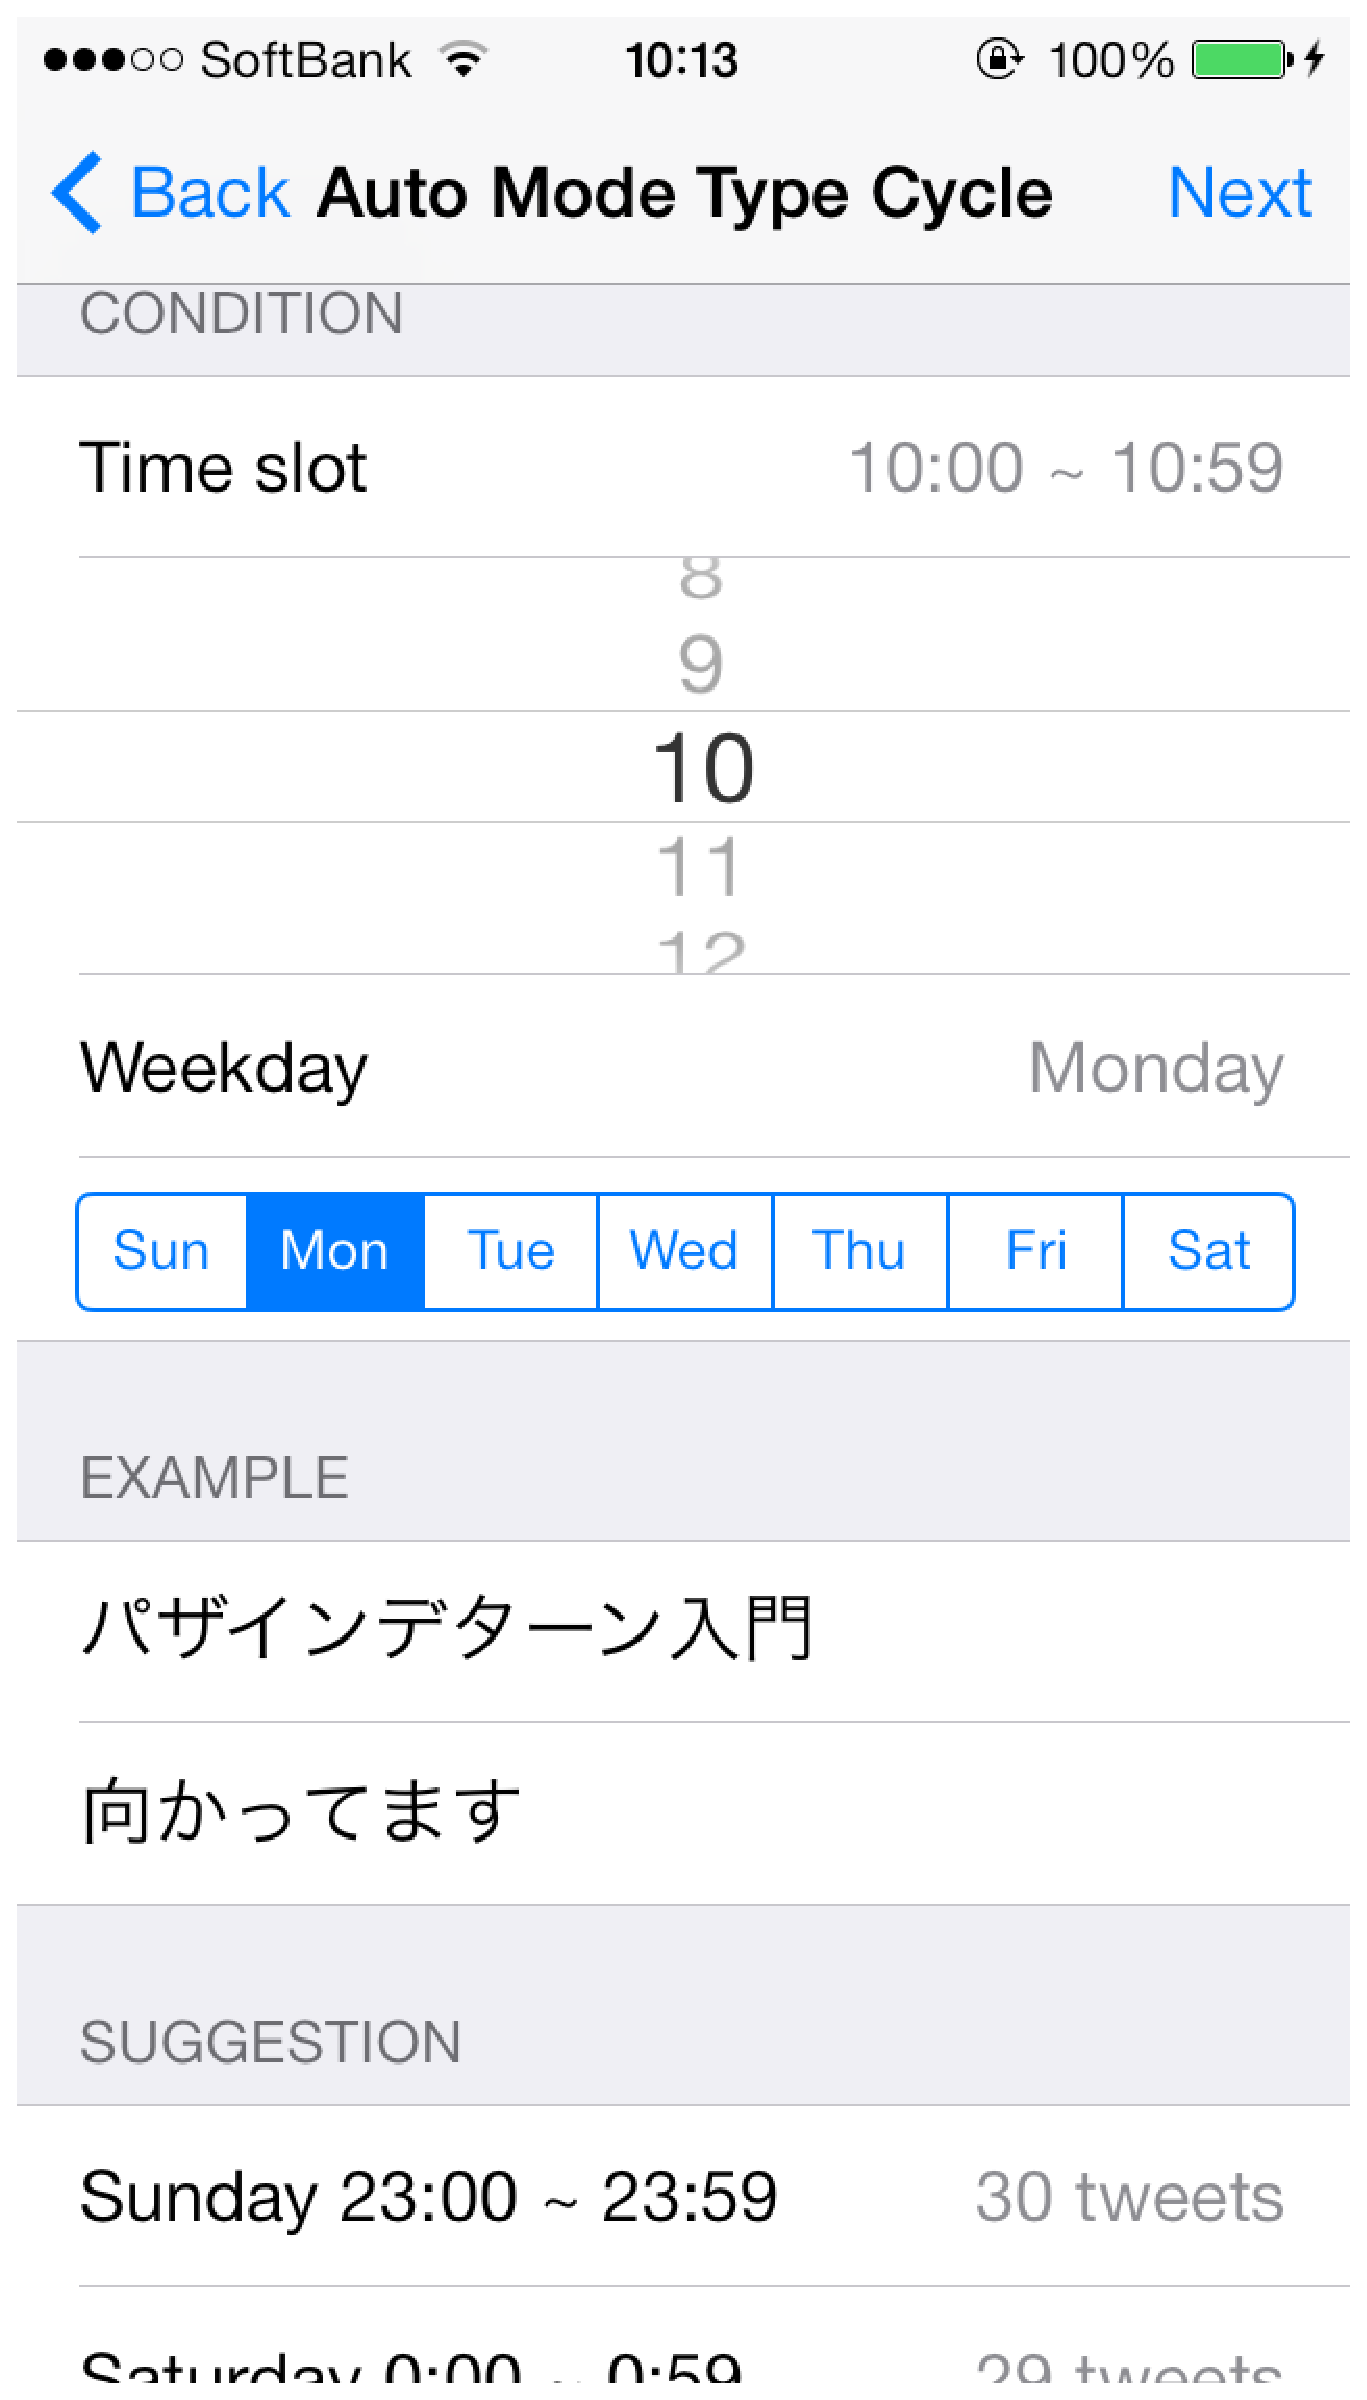
\includegraphics[width=60mm]{img/notifauthAutoCycle.eps}
  \end{center}
  \caption{Auto Mode Type Cycleの設定画面}
  \label{fig:notifauthAutoCycle}
\end{figure}

\subsubsection{具体例}
例えば,図\ref{fig:notifauthAutoCycle}に表示されているのと同じ,月曜日の10:00〜10:59に投稿されたツイートを秘密情報とするように設定すると,図\ref{fig:autoCycleSystem}のように,1/20時点で認証操作を行う際には,「今日はゼミだ」が秘密情報となるが,その2週間後である2/4に認証を行った時には「寝坊した!」も正しい秘密情報の一つとして追加され,「今日はゼミだ」と「寝坊した!」のどちらを選択しても認証は失敗する,という状況になる.

\subsection{Manual Mode}
この認証方式は,自分のツイート最新200件を取得し,その中から任意に1つ秘密情報となるものを選ぶ.
この方式では,認証時に新たなツイートの取得を行わないため,ダミーの選択肢は秘密情報を設定した時の群から選びぬかれる.

\subsubsection{意図}
当方式は3つの手法の中で最も単純であり,他の2つの方式のような特徴を持たない.
そのため,以下の欠点を抱えている.
\begin{itemize}
  \item 認証中の画面において,選択肢の中に必ず選択肢の一つとして表示されるため,総当たり攻撃や統計的手法を用いた攻撃に対して強度をもたない
\end{itemize}

\subsubsection{設定方法}
直近のツイートを最大200件取得し,これのうちどれを秘密情報とするかを図\ref{fig:notifauthManual}のように手動で選択し設定する.
ここで設定したツイートは,もう一度設定しない限りは実験終了まで固定されたままである.

\begin{figure}
  \begin{center}
    \includegraphics[width=60mm]{img/notifauthManual.eps}
  \end{center}
  \caption{Manual Modeの設定画面}
  \label{fig:notifauthManual}
\end{figure}

\section{認証操作}\label{sec:authentication}
第\ref{subsec:forMobile}節で述べたように,本システムでは認証操作にロック画面中の通知機能を利用し開発を行った.
実験を行いやすくするために本論文中の実装では,上記のロック画面を模した環境(図\ref{fig:notifauthTest})をアプリケーション内に実装した.

通知の表示画面を模した認証画面(図\ref{fig:notifauthTest}左)では,10個のツイートの本文と,当てはまるものがなかった場合に選択する「No match」の11つの候補を表示している.
その中から,正解だと思われるものを,指でタップし,そのまま右にスライドすることで,次の画面に遷移する.
なお,正解でないツイートの群をこれ以降,ダミーと呼ぶ.

PINの入力画面を模した認証画面(図\ref{fig:notifauthTest}右)では,0から9までのボタンと「キャンセル」ボタンが存在し,要求される桁数の入力が完了した段階で,結果画面に遷移する.
また,入力の途中で間違えた数字を選択してしまった場合は「キャンセル」ボタンをタップすることで,前画面に戻る.
その際,表示される候補の内容や順番は新たに更新される.

\begin{figure}[ht]
  \begin{center}
    \epsfig{file=img/notificationSliding.eps,scale=0.35}
  \end{center}
  \caption{ロック画面上における通知の選択(スライド)動作の例}
  \label{fig:notificationSliding}
\end{figure}

\begin{figure}[ht]
  \begin{minipage}{0.5\hsize}
    \begin{center}
      \includegraphics[width=60mm]{img/notifauthNotificationTest.eps}
    \end{center}
  \end{minipage}
  \begin{minipage}{0.5\hsize}
    \begin{center}
      \includegraphics[width=60mm]{img/notifauthPINTest.eps}
    \end{center}
  \end{minipage}
  \caption{左:ロック画面における通知の表示画面を模した認証画面,右:ロック画面におけるPINの入力画面を模した認証画面}
  \label{fig:notifauthTest}
\end{figure}

\section{システムの使用にあたって}
本システムを利用するための留意事項を表\ref{tbl:requirements}に記す.
本システムは,Apple社が開発した携帯端末向けオペレーティングシステムであるiOS 7を搭載している携帯端末を利用し,Twitterアカウントを保持していることが利用可能な最低条件となる.
加えて,1日あたりのツイートの数が極端に少ないと最低限度の安全性を保てない恐れが生じるため,定期的に複数のツイートを行っていることを推奨条件とした.
また,本アプリケーションは,OAuth\footnote{デスクトップ,モバイル,WebアプリケーションなどにセキュアなAPI認可の標準的手段を提供するためのオープンなプロトコル}を用いたTwitterとの連携を行わなければ利用することができない.

\begin{table}[htpb]
  \begin{center}
    \caption{留意事項}
    \label{tbl:requirements}
    \vspace{4mm}
    \begin{tabular}{ll}
    \bhline
    必要条件 & (1)iOS7を利用していること \\
     & (2)Twitterアカウントを保持していること \\
    推奨条件 & 定期的に複数のツイートを行っていること \\
    事前準備 & TwitterのOAuthを用いて本ソフトウェアと連携する \\
    \bhline
    \end{tabular}
  \end{center}
\end{table}

\section{開発環境}
本システムの開発環境を表\ref{tbl:environment}に示す.
本システムはApple社のパーソナルコンピュータ用OSであるMac OS Xと同社の総合開発環境であるXcodeを用いて開発を行った.
また,動作に必要なプラットフォームとして同社のiOSバージョン7.0以降を搭載している端末を要求し,サポート対象となっている現行機種の9割以上で動作の確認を行っている.
\begin{table}[htpb]
  \begin{center}
    \caption{開発環境}
    \label{tbl:environment}
    \vspace{4mm}
    \begin{tabular}{ll}
    \bhline
    プラットフォーム & Apple社 iOSバージョン7.0以上 \\
    開発言語 & Objective-C \\
    実装環境 & Mac OS X 10.9, Xcode5 \\
    動作確認環境 & iPhone 4,iPhone 4S,iPhone 5,iPhone 5S,iPod touch \\
    \bhline
    \end{tabular}
  \end{center}
\end{table}

\newpage

%実験
\chapter{検証実験}\label{chap:experiment}

\section{概要}
本論文で提案する個人認証システムについて,以下の3つの評価実験を行った.
\begin{description}
  \item[Manual Modeを用いた認証方式の評価実験] SNSの情報を利用することで,従来のPINを一桁増やした認証と比較し,どれだけ利便性と安全性を向上させることができるかを検証する
  \item[Auto Mode Type Termを用いた認証方式の評価実験] 一定のルール(期間)に基づいて秘密情報が変化することが認証の成功率やユーザへの負担にどう影響を与えるかについて検証する
  \item[Auto Mode Type Cycleを用いた認証方式の評価実験] 一定のルール(周期)に基づいて秘密情報が変化することが認証の成功率やユーザへの負担にどう影響を与えるかについて検証する
\end{description}
それぞれの実験は,時間的な制約から予備実験,本実験などの形式で行うことをせず,一度に行った.
また,ユーザからみた利便性に対する評価を得るするため,2回の選択式(一部自由記述含む)アンケートを実施した.

\subsection{実験手順}
以降の節のそれぞれの実験は第\ref{subsec:selectSecret}節にて挙げた3つの実装(以降,「パターン」と記載する)に対応しており,それぞれのパターンは多要素化手法として評価するために認証操作の後に4桁のPINによる認証操作を追加した.
そこに「PINの桁数を一桁増やし,5桁にしたものを秘密情報とする」パターンを追加し,計4パターンで相互に比較を行った.
各パターンの実験は一つにつき8日間にわたって実施,その間に設定した日から数えて,0日目(設定直後),1日目,3日目,8日目の4回の認証試行を行った(図\ref{fig:schedule}).
それぞれのパターンで実験中の期間は重複せず,順番は偏りのないように設定し,そのスケジュールにそって全実験を実施した.
また,アンケートに関しては,16日目が経過した段階で,2種類のパターンを比較するための中間アンケート(付録\ref{apdx:interimEnquete})を,32日目が経過した段階で最終アンケート(付録\ref{apdx:finalEnquete})を行った.
\footnote{スケジュールは4つのパターンの組み合わせであり,その総数は$ {}_4 P _4 $の式で表される.
本実験ではこれら全てに固有の番号(以降,「スケジュール番号」と記載する)を付録\ref{apdx:schedule}の通り割り振って管理する.}

\begin{figure}[ht]
  \begin{center}
    \epsfig{file=img/schedule.pdf,scale=1.1}
  \end{center}
  \caption{実験スケジュール}
  \label{fig:schedule}
\end{figure}

\subsubsection{初回実験説明・導入}
\begin{enumerate}
  \item 実験担当者が実験の目的・注意事項・免責事項を説明する.この手順は付録\ref{apdx:experiment}の実験説明資料と操作説明資料を用いて行い,不明な点があれば質問してもらった.
  \item 被験者のスケジュールを決定し,それに合わせて提案システムを実装したアプリケーションソフトウェア(以降「Notifauth」と記載する)のソースコードにスケジュール番号を登録した.
  \item 実験担当者の開発用端末と被験者の携帯端末を接続し,Notifauthをインストールする\footnote{ここでAppleの開発者用アカウントと被験者の端末の紐付けを行う}.
  \item 実際にNotifauthを操作し,全てのパターンでひと通りの秘密情報設定と認証操作を行ってもらった.
  \item その後,Notifauth内の全ての保存されたデータを初期化し,スケジュールに沿ったパターンのみ設定を行ってもらうことで実験開始とした.
  \item 上記手順で設定したパターンについて認証操作を行ってもらった.
  \item この段階で実験データを送信してもらい,該当データの受信を実験担当者が確認を行った.
\end{enumerate}

\subsubsection{試行手順}
\begin{enumerate}
  \item トップ画面(付録\ref{apdx:screen}内の図\ref{fig:notifauthHome})で,試行したいパターンをセレクタで選択し,「Test」をタップする.
  \item ``PIN Mode''以外の場合,ロック画面を模した画面(第\ref{sec:authentication}内の図\ref{fig:notifauthTest}左図)が表示され,秘密情報に当てはまると思われるツイートを見つけ,そのセルをスライドする.
  \item PINの入力画面(第\ref{sec:authentication}内の図\ref{fig:notifauthTest}右図)が表示され,``PIN Mode''であれば5桁,それ以外のパターンであれば4桁のPINを入力する.
  \item 結果画面が表示されるので,「Home」ボタンを押する.
\end{enumerate}

なお,試行手順の一つとして、実験結果は認証操作直後にメールで送信して頂くかたちで収集した.

\subsection{被験者}
男性12名,女性3名の計15名が実験を行った.
うち本学の学生は5名であった.
性別や年齢は表\ref{fig:participants}の通りである.
全ての検証実験を終了したのは11人で,そのうち最終アンケートに答えたのは5人である.
中間アンケートには12人が回答した.

\begin{figure}[ht]
  \begin{minipage}{0.32\hsize}
    \begin{center}
      \includegraphics[width=40mm]{resource/users_gender.pdf}
    \end{center}
  \end{minipage}
  \begin{minipage}{0.32\hsize}
    \begin{center}
      \includegraphics[width=50mm]{resource/users_age.pdf}
    \end{center}
  \end{minipage}
  \begin{minipage}{0.32\hsize}
    \begin{center}
      \includegraphics[width=50mm]{resource/users_tweet.pdf}
    \end{center}
  \end{minipage}
  \caption{被験者の特性(左:性別,中央:年齢,右:1日あたりのツイート数)}
  \label{fig:participants}
\end{figure}

%\begin{table}[ht]
%  \caption{被験者の特性}
%  \label{tab:participants}
%  \begin{minipage}{0.25\hsize}
%    \begin{center}
%      \small
%      \begin{tabular}{lr}
%        \bhline
%        \multicolumn{2}{l}{性別} \\ \hline
%        男性 & 15 \\
%        女性 & 3 \\
%        \bhline
%      \end{tabular}
%    \end{center}
%  \end{minipage}
%  \begin{minipage}{0.25\hsize}
%    \begin{center}
%      \small
%      \begin{tabular}{lr}
%        \bhline
%        \multicolumn{2}{l}{年齢} \\ \hline
%        10代 & 0 \\
%        20代 & 12 \\
%        30代 & 2 \\
%        40代 & 1 \\
%        50代以上 & 0 \\
%        \bhline
%      \end{tabular}
%    \end{center}
%  \end{minipage}
%  \begin{minipage}{0.25\hsize}
%    \begin{center}
%      \small
%      \begin{tabular}{lr}
%        \bhline
%        \multicolumn{2}{l}{1日の平均ツイート数} \\ \hline
%        0〜1 & 0 \\
%        2〜10 & 0 \\
%        11〜50 & 0 \\
%        50〜100 & 0 \\
%        100〜 & 0 \\
%        \bhline
%      \end{tabular}
%    \end{center}
%  \end{minipage}
%\end{table}

\section{Manual Modeを用いた認証方式の評価実験}\label{sec:vsTweet}
\subsection{概要}
本実験では,SNSの情報を利用することで,従来のPINを一桁増やした認証と比較し,どれだけ利便性と安全性を向上させることができるかの評価を行う.
本実験で評価対象とするパターンとして,``Manual Mode''を採用する.

\subsection{目的}
アプリケーションを用いた実験では,測定した結果から以下の3指標にもとづいて相関や有意差をみた.
\begin{itemize}
  \item 短期の記憶保持
    \begin{description}
      \item[目的] 秘密情報の短期記憶が可能かどうかの検証
      \item[仮説] 日数をおかない試行において5桁のPIN認証よりも認証成功率が高い,つまり,短期の記憶保持について暗証番号認証よりも当方式を用いた認証の方が容易
      \item[測定方法] 0日目,1日目,3日目の認証成功率を比較し,相関をみる
    \end{description}
  \item 長期の記憶保持
    \begin{description}
      \item[目的] 秘密情報の長期記憶が可能かどうかの検証
      \item[仮説] 日数をおく試行において5桁のPIN認証よりも認証成功率が高い,つまり,長期の記憶保持について暗証番号認証よりも当方式を用いた認証の方が容易
      \item[測定方法] 3日目と8日目の認証成功率を比較し,相関をみる.
    \end{description}
  \item 認証時間
    \begin{description}
      \item[目的] 利便性の検証
      \item[仮説] 5桁のPIN認証よりも認証時間が短い,つまり,暗証番号認証よりも当方式を用いた認証の方が利便性が高い
      \item[測定方法] 認証操作の画面が表示されてから,認証を終えるまでの時間を計測する.認証の成否は問わないものとする.
    \end{description}
\end{itemize}

\subsection{方法}
被験者実験により各試行の成功と失敗,認証にかかった時間を収集し,事後アンケートを実施する.
また,有意差はWelchのt検定を用いる(この場合,(1)サンプルサイズが30以上で十分大きいこと,(2)検定を複数回繰り返すことで帰無仮説全体を通しての有意水準が不当に上昇してしまう,(3)t検定は母分布が正規分布でないときにも頑健性を持つ(妥当な結果を与える),ことから,標本が正規分布であることは検証をせずに自明とした.

\subsection{結果}
本実験の結果を表\ref{tab:manual.data}に示す.
試行のタイミングが1日程度前後した被験者が存在したため,1〜2日目を1日目,3〜6日目におこなったものを3日目,7〜8日目に行ったものを8日目の試行とした.
比較のためのPIN Modeにおける認証成功率と認証時間は表\ref{tab:manual.data}に示す.

\begin{table}[t]
  \caption{Manual Modeにおける各経過日数ごとの認証成功率と認証時間の変化($ n = 39 $)}
  \label{tab:manual.data}
  \begin{center}
    \small
    \begin{tabular}{rrr}
      \bhline
      経過日数 & 認証成功率(\%) & 認証時間(秒)\\ \hline
      0 & 90.0 & 17.05 \\
      1〜2 & 88.9 & 11.86 \\
      3〜6 & 88.9 & 9.82 \\
      7〜8 & 100.0 & 10.11 \\ \hline \hline
      平均 & 91.89 & 12.34 \\
      標準偏差 & 4.67 & 9.56 \\
      中央値 & & 8.67 \\
      最大値 & & 41.84 \\
      最小値 & & 3.29 \\
      \bhline
    \end{tabular}
  \end{center}
\end{table}

\begin{table}[b]
  \caption{PIN Modeにおける各経過日数ごとの認証成功率と認証時間の変化($ n = 45 $)}
  \label{tab:manual.data}
  \begin{center}
    \small
    \begin{tabular}{rrr}
      \bhline
      経過日数 & 認証成功率(\%) & 認証時間(秒)\\ \hline
      0 & 100.0 & 2.24 \\
      1〜2 & 100.0 & 2.76 \\
      3〜6 & 90.00 & 2.70 \\
      7〜8 & 100.0 & 2.51 \\ \hline \hline
      平均 & 97.78 & 2.54 \\
      標準偏差 & 4.33 & 1.66 \\
      中央値 & & 1.92 \\
      最大値 & & 8.40 \\
      最小値 & & 1.11 \\
      \bhline
    \end{tabular}
  \end{center}
\end{table}

\begin{figure}[t]
  \begin{center}
    \epsfig{file=resource/ex_manual_vs_pin_rate.pdf,scale=0.5}
  \end{center}
  \caption{Manual ModeとPIN Modeにおける設定時からの経過日数ごとの認証成功率}
  \label{fig:ex_manual_vs_pin_rate}
\end{figure}

\begin{figure}[b]
  \begin{center}
    \epsfig{file=resource/ex_manual_vs_pin_time.pdf,scale=0.5}
  \end{center}
  \caption{Manual ModeとPIN Modeにおける設定時からの経過日数ごとの認証時間}
  \label{fig:ex_manual_vs_pin_time}
\end{figure}

\subsubsection{記憶保持}
表\ref{tab:manual.data}に示した通り,経過日数と認証成功率におけるピアソンの相関係数は0.8813で,標本数による限界値\cite{978-4641121607}を考慮しても有意な差ではないと考えられる.
また,図\ref{fig:ex_manual_vs_pin_rate}にPIN Modeとの認証率の比較を示した.
検定を行った結果,PIN Modeの認証成功率とは有意差がある(Welchのt検定,$ p = 0 $)ことが明らかになった.

\begin{itemize}
  \item 短期の記憶保持
\end{itemize}
0日目,1日目,3日目にかけてのManual Modeでの認証成功率は90.0\%,88.89\%,90.0\%と推移しており,ピアソン相関係数は0.048であった.

\begin{itemize}
  \item 長期の記憶保持
\end{itemize}
3日目の認証成功率は90\%で,8日目には100\%であった.
3日目から8日目にかけてのピアソン相関係数は0.274であった.

\subsubsection{認証時間}
図\ref{fig:ex_manual_vs_pin_time}にManual ModeとPIN Modeとの認証時間の比較を示した.
PIN Modeとは数値上4倍程度の差があり,検定を行った結果,有意差がある(Welchのt検定,$ p = 0 $)といえた.

\subsubsection{アンケート結果}
以下に被験者によるアンケート結果を示す.
試行のタイミングが1日程度前後した被験者が存在したため,1〜2日目を1日目,3〜6日目におこなったものを3日目,7〜8日目に行ったものを8日目の試行とした.
比較のためのPIN Modeにおける認証成功率と認証時間は第\label{sec:vsManual}節と同じく表\ref{tab:manual.data}に示す.
\begin{table}[t]
  \caption{被験者によるManual Modeに対するアンケート内評価}
  \label{tab:manual.enquete}
  \begin{center}
    \small
    \begin{tabular}{lrr}
      \bhline
      項目名(とても小さい:1〜とても大きい:5) & 平均値 & 回答者数 \\ \hline
      秘密情報の記憶保持にかかわる負担はどのくらい感じますか? & 1.13 & 8 \\
      認証にかかる時間はどのように感じましたか? & 1.13 & 8 \\
      認証を成功させるために必要な操作負担はどの程度でしたか? & 1.25 & 8 \\
      認証を行うのにどれくらいフラストレーションを感じましたか? & 1.5 & 8 \\
      タイピングしたりタッチパネルをスライドしたりする作業の負担はどの程度でしたか? & 1.43 & 7 \\
      \bhline
    \end{tabular}
  \end{center}
\end{table}
\begin{table}[b]
  \caption{被験者によるPIN Modeに対するアンケート内評価}
  \label{tab:pin.enquete}
  \begin{center}
    \small
    \begin{tabular}{lrr}
      \bhline
      項目名(とても小さい:1〜とても大きい:5) & 平均値 & 回答者数 \\ \hline
      秘密情報の記憶保持にかかわる負担はどのくらい感じますか? & 1.13 & 8 \\
      認証にかかる時間はどのように感じましたか? & 1.13 & 8 \\
      認証を成功させるために必要な操作負担はどの程度でしたか? & 1.13 & 8 \\
      認証を行うのにどれくらいフラストレーションを感じましたか? & 1.5 & 8 \\
      タイピングしたりタッチパネルをスライドしたりする作業の負担はどの程度でしたか? & 1.43 & 7 \\
      \bhline
    \end{tabular}
  \end{center}
\end{table}

\section{Auto Mode Type Termを用いた認証方式の評価実験}\label{sec:vsTerm}
\subsection{概要}
本実験では,SNSの情報の特性を利用した認証システムとして``Auto Mode Type Term''を採用し,記憶持続性と利便性の評価を行う.
更に,ある一定のルールに基づいて秘密情報が変化することが認証の成功率やユーザへの負担がどう影響を与えるかについても検証する.
また,他の実験で用いたパターンとの比較も行う.

\subsection{目的}
アプリケーションを用いた実験で測定した結果から相関や有意差をみた指標は第\ref{sec:vsTweet}節に準じ,(1)短期の記憶保持,(2)長期の記憶保持,(3)認証時間とした.

\subsection{方法}
被験者実験により各試行の成功と失敗,認証にかかった時間を収集し,事後アンケートを実施する.
平均値を比較する際の検定方法は\ref{sec:vsTweet}節に準じ,Welchのt検定を利用した.

\subsection{結果}
本実験の結果を表\ref{tab:auto_term.data}に示す.
試行のタイミングが1日程度前後した被験者が存在したため,1〜2日目を1日目,3〜6日目におこなったものを3日目,7〜8日目に行ったものを8日目の試行とした.
比較のためのPIN Modeにおける認証成功率と認証時間は第\label{sec:vsManual}節と同じく表\ref{tab:manual.data}に示す.
\begin{table}[ht]
  \caption{Auto Mode Type Termにおける各経過日数ごとの認証成功率と認証時間の変化}
  \label{tab:auto_term.data}
  \begin{center}
    \small
    \begin{tabular}{rrr}
      \bhline
      経過日数 & 認証成功率(\%) & 認証時間\\ \hline
      0 & 46.15 & 21.04 \\
      1〜2 & 44.44 & 17.62 \\
      3〜6 & 80.00 & 16.29 \\
      7〜8 & 62.50 & 14.22 \\ \hline \hline
      平均 & 61.36 & 19.81 \\
      標準偏差 & 14.39 & 13.03 \\
      中央値 & & 16.95 \\
      最大値 & & 65.02 \\
      最小値 & & 5.62 \\
      \bhline
    \end{tabular}
  \end{center}
\end{table}

\begin{figure}[ht]
  \begin{center}
    \epsfig{file=resource/ex_auto_term_vs_pin_rate.pdf,scale=0.5}
  \end{center}
  \caption{Auto Mode Type TermとPIN Modeにおける設定時からの経過日数ごとの認証成功率}
  \label{fig:ex_auto_term_vs_pin_rate}
\end{figure}

\begin{figure}[hb]
  \begin{center}
    \epsfig{file=resource/ex_auto_term_vs_pin_time.pdf,scale=0.5}
  \end{center}
  \caption{Auto Mode Type TermとPIN Modeにおける設定時からの経過日数ごとの認証時間}
  \label{fig:ex_auto_term_vs_pin_time}
\end{figure}

\subsubsection{記憶保持}
表\ref{tab:auto_term.data}に示した通り,経過日数と認証成功率におけるピアソンの相関係数は0.8813で,標本数による限界値を考慮すると有意ではないと考えられる.
また,図\ref{fig:ex_auto_term_vs_pin_rate}にPIN Modeとの認証率の比較を示した.
検定を行った結果,PIN Modeの認証成功率とは有意差がある(Welchのt検定,p=0)ことが明らかになった.
\begin{itemize}
  \item 短期の記憶保持
\end{itemize}
0日目から3日目までのManual Modeでの認証成功率は50.00\%から85.71\%とばらつきがみられ,ピアソン相関係数は0.277で有意な相関ではない.

\begin{itemize}
  \item 長期の記憶保持
\end{itemize}
3日目の認証成功率は85\%,8日目の認証成功率は66.67\%で,期間が空くと認証成功率が下がってしまった.
3日目から8日目の期間におけるピアソン相関係数は0.177で,相関はみられなかった.

\subsubsection{認証時間}
図\ref{fig:ex_auto_term_vs_pin_time}にPIN Modeとの認証時間の比較を示した.
こちらもManual Mode同様,PIN Modeとは大きく差があり,検定を行った結果,有意差がある(Welchのt検定,$ p = 0 $)ことが判明した.

\subsubsection{アンケート結果}
被験者によるアンケート結果を表\ref{tab:auto_term.enquete}に記す.
\begin{table}[ht]
  \caption{被験者によるAuto Mode Type Termに対するアンケート内評価}
  \label{tab:auto_term.enquete}
  \begin{center}
    \small
    \begin{tabular}{lrr}
      \bhline
      項目名(とても小さい:1〜とても大きい:5) & 平均値 & 回答者数 \\ \hline
      秘密情報の記憶保持にかかわる負担はどのくらい感じますか? & 4.09 & 11 \\
      認証にかかる時間はどのように感じましたか? & 3.73 & 11 \\
      認証を成功させるために必要な操作負担はどの程度でしたか? & 3.18 & 11 \\
      認証を行うのにどれくらいフラストレーションを感じましたか? & 3.45 & 11 \\
      タイピングしたりタッチパネルをスライドしたりする作業の負担はどの程度でしたか? & 3.14 & 7 \\
      \bhline
    \end{tabular}
  \end{center}
\end{table}

\section{Auto Mode Type Cycleを用いた認証方式の評価実験}\label{sec:vsCycle}
\subsection{概要}
本実験では,SNSの情報の特性を利用した認証システムとして``Auto Mode Type Cycle''を採用し,記憶持続性と利便性の評価を行う.
更に,ある一定のルールに基づいて秘密情報が変化することが認証の成功率やユーザへの負担がどう影響を与えるかについても検証する.
また,他の実験で用いたパターンとの比較も行う.

\subsection{目的}
アプリケーションを用いた実験で測定した結果から相関や有意差をみた指標は第\ref{sec:vsTweet}節に準じ,(1)短期の記憶保持,(2)長期の記憶保持,(3)認証時間とした.

\subsection{方法}
被験者実験により各試行の成功と失敗,認証にかかった時間を収集し,事後アンケートを実施する.
平均値を比較する際の検定方法は\ref{sec:vsTweet}節に準じ,Welchのt検定を利用した.

\subsection{結果}
本実験の結果を表\ref{tab:auto_cycle.data}に示す.
試行のタイミングが1日程度前後した被験者が存在したため,1〜2日目を1日目,3〜6日目におこなったものを3日目,7〜8日目に行ったものを8日目の試行とした.
比較のためのPIN Modeにおける認証成功率と認証時間は第\label{sec:vsManual}節と同じく表\ref{tab:manual.data}に示す.
\begin{table}[ht]
  \caption{Auto Mode Type Cycleにおける各経過日数ごとの認証成功率と認証時間の変化}
  \label{tab:auto_cycle.data}
  \begin{center}
    \small
    \begin{tabular}{rrr}
      \bhline
      経過日数 & 認証成功率(\%) & 認証時間\\ \hline
      0 & 33.33 & 20.84 \\
      1〜2 & 18.18 & 20.42 \\
      3〜6 & 11.11 & 36.56 \\
      7〜8 & 12.50 & 24.19 \\ \hline \hline
      平均 & 21.95 & 2.54 \\
      標準偏差 & 8.81 & 16.03 \\
      中央値 & & 20.22 \\
      最大値 & & 91.03 \\
      最小値 & & 5.87 \\
      \bhline
    \end{tabular}
  \end{center}
\end{table}

\begin{figure}[t]
  \begin{center}
    \epsfig{file=resource/ex_auto_cycle_vs_pin_rate.pdf,scale=0.5}
  \end{center}
  \caption{Auto Mode Type CycleとPIN Modeにおける設定時からの経過日数ごとの認証成功率}
  \label{fig:ex_auto_cycle_vs_pin_rate}
\end{figure}

\begin{figure}[b]
  \begin{center}
    \epsfig{file=resource/ex_auto_cycle_vs_pin_time.pdf,scale=0.5}
  \end{center}
  \caption{Auto Mode Type CycleとPIN Modeにおける設定時からの経過日数ごとの認証時間}
  \label{fig:ex_auto_cycle_vs_pin_time}
\end{figure}

\subsubsection{記憶保持}
表\ref{tab:auto_cycle.data}に示した通り,経過日数と認証成功率におけるピアソンの相関係数は0.8813で,標本数による限界値を考慮すると有意ではないと考えられる.
また,図\ref{fig:ex_auto_cycle_vs_pin_rate}にPIN Modeとの認証率の比較を示した.
検定を行った結果,PIN Modeの認証成功率とは有意差がある(Welchのt検定,p=0)ことが明らかになった.
\begin{itemize}
  \item 短期の記憶保持
\end{itemize}
0日目から3日目までのAuto Mode Type Cycleにおける認証成功率は33.00\%から0\%まで落ちた.
この期間でのピアソン相関係数は-0.121であった.

\begin{itemize}
  \item 長期の記憶保持
\end{itemize}
3日目の認証成功率は0\%,8日目の認証成功率は16.67\%であり,ピアソン相関係数は0.142であった.

\subsubsection{認証時間}
図\ref{fig:ex_auto_cycle_vs_pin_time}にPIN Modeとの認証時間の比較を示した.
こちらも他のMode同様,PIN Modeとは大きく差があり,検定を行った結果,有意差がある(Welchのt検定,p=0)ことが判明した.

\subsubsection{アンケート結果}
被験者によるアンケート結果を表\ref{tab:auto_cycle.enquete}に記す.
\begin{table}[ht]
  \caption{被験者によるAuto Mode Type Cycleに対するアンケート内評価}
  \label{tab:auto_cycle.enquete}
  \begin{center}
    \small
    \begin{tabular}{lrr}
      \bhline
      項目名(とても小さい:1〜とても大きい:5) & 平均値 & 回答者数 \\ \hline
      秘密情報の記憶保持にかかわる負担はどのくらい感じますか? & 3.56 & 9 \\
      認証にかかる時間はどのように感じましたか? & 3.44 & 9 \\
      認証を成功させるために必要な操作負担はどの程度でしたか? & 2.44 & 9 \\
      認証を行うのにどれくらいフラストレーションを感じましたか? & 3.44 & 9 \\
      タイピングしたりタッチパネルをスライドしたりする作業の負担はどの程度でしたか? & 2.57 & 7 \\
      \bhline
    \end{tabular}
  \end{center}
\end{table}

%\section{各評価実験間での相互比較}\label{sec:vsAll}
%\subsection{目的}
%本節では,各評価実験で行ったパターン全てのなかで比較を行う.%

%\subsection{方法}
%被験者実験により各試行の成功と失敗,認証にかかった時間を収集する.
%また,付録の\ref{apdx:interimEnquete}や\ref{apdx:finalEnquete}にある通り,被験者には使用パターンについて5段階のリッカート尺度を使った質問に答えてもらい,さらに既に8日間の試行が終了している他パターンとの比較もしてもらう.%

%\subsection{結果}
%\subsubsection{期間と周期での比較}
%図\ref{fig:ex_auto_term_vs_auto_cycle_rate}と図\ref{fig:ex_auto_term_vs_auto_cycle_time}にAuto Modeの2タイプにおけるそれぞれの経過日数ごとの認証成功率と認証時間を示す.
%認証の成功率に関しては,有意差が見られた(Welchのt検定においてp=0).
%認証の成功時間に関しては,有意な差は見られなかった(Welchのt検定においてp=0.508).%

%\begin{figure}[ht]
%  \begin{center}
%    \epsfig{file=resource/ex_auto_term_vs_auto_cycle_rate.pdf,scale=0.5}
%  \end{center}
%  \caption{Auto Mode Type TermとAuto Mode Type Cycleにおける設定時からの経過日数ごとの認証成功率}
%  \label{fig:ex_auto_term_vs_auto_cycle_rate}
%\end{figure}%

%\begin{figure}[ht]
%  \begin{center}
%    \epsfig{file=resource/ex_auto_term_vs_auto_cycle_time.pdf,scale=0.5}
%  \end{center}
%  \caption{Auto Mode Type TermとAuto Mode Type Cycleにおける設定時からの経過日数ごとの認証時間}
%  \label{fig:ex_auto_term_vs_auto_cycle_time}
%\end{figure}%

%アンケートによる比較結果を図\ref{tab:term_vs_cycle.enquete}に示す.%

%\begin{table}[ht]
%  \begin{center}
%    \small
%    \begin{tabular}{lr}
%      \bhline
%      \multicolumn{2}{l}{どちらのパターンの方が認証操作が楽でしたか?} \\\hline
%      Auto Mode Type Term (\%) & 20 \\
%      Auto Mode Type Cycle (\%) & 5 \\ \hline \hline
%      \multicolumn{2}{l}{どちらのパターンの方が秘密保持しやすかったですか?} \\ \hline
%      Auto Mode Type Term (\%) & 20 \\
%      Auto Mode Type Cycle (\%) & 5 \\ \hline \hline
%      \multicolumn{2}{l}{今後日常的に使わなければならないとすれば,どちらのパターンを使いたいですか?} \\ \hline
%      Auto Mode Type Term (\%) & 20 \\
%      Auto Mode Type Cycle (\%) & 5 \\
%      \bhline
%    \end{tabular}
%  \end{center}
%  \caption{被験者によるAuto Mode Type TermとAuto Mode Type Cycleの比較[NOTICE: 未確定]}
%  \label{tab:term_vs_cycle.enquete}
%\end{table}

%\subsubsection{4つ全ての比較}
%アンケートによる比較結果を図\ref{tab:vs_all.enquete}に示す.
%被験者の○割以上が,△△による設定の方が使いやすさ,覚えやすさ共に優れていると判断した.

%\begin{table}[ht]
%  \begin{center}
%    \small
%    \begin{tabular}{lr}
%      \bhline
%      \multicolumn{2}{l}{どのパターンが最も認証操作が楽でしたか?} \\ \hline
%      Auto Mode Type Term (\%) & 20 \\
%      Auto Mode Type Cycle (\%) & 5 \\
%      Manual Mode (\%) & 30 \\
%      PIN Mode (\%) & 45 \\ \hline \hline
%      \multicolumn{2}{l}{どのパターンが最も秘密保持しやすかったですか?} \\ \hline
%      Auto Mode Type Term (\%) & 20 \\
%      Auto Mode Type Cycle (\%) & 5 \\
%      Manual Mode (\%) & 30 \\
%      PIN Mode (\%) & 45 \\ \hline \hline
%      \multicolumn{2}{l}{今後日常的に使わなければならないとすれば,どのパターンを最も使いたいですか?} \\ \hline
%      Auto Mode Type Term (\%) & 20 \\
%      Auto Mode Type Cycle (\%) & 5 \\
%      Manual Mode (\%) & 30 \\
%      PIN Mode (\%) & 45 \\
%      \bhline
%    \end{tabular}
%  \end{center}
%  \caption{被験者による全パターンにおける比較[NOTICE: 未確定]}
%  \label{tab:vs_all.enquete}
%\end{table}

\newpage


%考察
\chapter{考察}\label{chap:discussion}
\section{安全性に関する考察}\label{sec:safety}
安全性に関しては,単純な場合の数においては5桁のPINによる認証方式と同等の$ 10 ^ 5 $通りにして実験を行い,認証要素を増やす前と比べて安全性が向上したと言える.
また,本システムでは,ダミーの数を増やすことで柔軟に安全性を高めることができる.
しかし,設定情報が漏洩してしまえば,あとは使用しているアカウントの投稿データを取得するだけで簡単に攻撃が可能となってしまう.
加えて,期間や周期を秘密情報として設定を行う場合,設定情報のエントロピーは投稿の頻度に依存し,従来の方式に比べて高いとはいえない.

更に,認証のエラー率を下げるために秘密情報が極端に多いまたは小さくなるよう設定した場合にも統計を用いた攻撃に脆弱となってしまう恐れがある.
そのため,設定時の因子を増やしたり,認証操作をリストからの選択式にせず2択を用いた上で回答回数を増やすなどの改善によってエントロピーを減少させず\cite{kaneko:2013-01-22}にエラー率を低下させる方法を検討する必要があると考えられる.

\section{覚えやすさに関する考察}\label{sec:memorable}
本システムの認証方式では,Twitterの投稿を用いることによって覚えやすさを向上させることが主たる目的として存在し,被験者実験において,Manual Modeによる手動での秘密情報の設定の場合は5桁のPINによる認証と比べても同等の認証成功率を得ることができたと考えられる.

Auto Mode Type Termにおいて,0日目から3日目までのManual Modeでの認証成功率において,その中で0日目と1日目の認証成功率が低いにも関わらず3日目で上昇しており,設定した条件は記憶していたもののうまく候補の中から当てることが出来なかった可能性がある.
Auto Mode Type Cycleにおいては,8日間通しての平均認証成功率は27.59\%と,PINによる認証と比べてかなり劣ることが明らかになったが,この結果に関しても上記の理由によるものだと推測できる.
それらの条件設定により秘密情報が変化する手法では,設定は覚えているがその条件に当てはまる秘密情報を選ぶことができない場合が多かったことは第\ref{sec:vsTerm}節と第\ref{sec:vsCycle}節のアンケートの結果からもみることができた.
そのため,ユーザの記憶が曖昧になってしまうと考えられる情報を排除するなどの対策をとる必要があると考えられる.

長期間における記憶に関しては,Auto Mode Type Termに関しては75.0\%から41.7\%と認証成功率の大幅な下降がみられたが,それ以外の認証方式では大きく下降しないもしくは大きく上昇し,Auto Mode Type Termに関しても有意な相関ではないことと前段落の推測から,いずれの方式も覚えやすさに大きな差はないと考えられる.

3つの提案手法と1つの既存手法を比較すると,42.9\%の被験者がManual Modeが最も覚えやすいと答え,同じく28.6\%の被験者はPIN Modeが最も覚えやすいと答えた.
そのため,Manual Modeに関してはPINよりも覚えやすさにおいて優れていると言える.

\section{使用継続性に関する考察}\label{sec:continuity}
本システムの認証方式では,設定方法によっては長期間使用することにより,秘密情報のエントロピーが上昇したり,自動的に秘密情報が入れ替わることで定期的な秘密情報変更をする必要が小さくなるなどの利点が存在する.
また,被験者アンケートで得られた感想などを見ても,利便性についての評価が高かった.
しかしながら,認証操作にかかる時間に関しては,いずれの方式もPINによる認証よりも平均で10倍以上も多くかかっているという結果が得られているため,日常的に頻繁に使用する携帯端末においては,ユーザの利便性を著しく下げ,利用継続性を損ねてしまう可能性が存在する.
この問題点の解決方法として,既存研究のように認証手法を2択にして複数回回答させるといったものが挙げられる.

3つの提案手法と1つの既存手法を比較すると,57.1\%の被験者がManual Modeが最も「今後日常的に使いたい」と答え,PIN Modeでそう答えた被験者は28.6\%であった.
そのため,Manual Modeに関してはPINよりも使用継続性において優れていると言える.

\section{他環境における応用に関する考察}\label{sec:application}
本システムの考え方は,ハードウェアへの依存の少なさや,設定方法の単純さから,携帯端末以外の環境でも応用が可能だと考えられる.

また,他のSNSを使用可能かという点に関しては,OAuthなどのセキュアな認証プロトコルとWeb APIが提供されていればデータベース構造などを大きく変える必要もなく導入できる.
これにより,様々なSNSの情報を組み合わせることでエントロピーの上昇や,新たな秘密情報の設定が可能になることで安全性の向上にも繋がることが考えられる.

\section{今後の課題}
\subsection{仕組み}
認証時に表示する秘密情報の候補数は,総当たり攻撃に対する頑強さに直結する.
そのため,どれくらいの数まで候補を表示しても,ユーザが負担だと感じないかを調べる必要があり,それによってユーザの利便性を可能な限り損なわない形で簡単に安全性を強化できると考えられる.

秘密情報の設定において,アンケートで得られた回答として多かったのは,「設定情報は覚えているがそれに当てはまるツイートを選べない」という問題である.
これが原因で,自動で設定する2手法(Auto Mode Type TermとAuto Mode Type Cycle)では,大きく認証成功率が落ちていると考えられる.
また,本手法においては,被験者が任意に条件を設定することが可能なので,認証成功率が低くなれば自然に簡単な設定,例えば「Fromを1年前,Termを1年間に設定する(直近1年間のツイート全てが秘密情報となる)」や「明け方など,1-2件しかツイートしていない時間帯にTime slotを設定(そのツイートの内容自体を覚えてしまう)」などにしがちであると予測できる.
これは被験者実験によって得られた設定内容からも読み取ることができ,これにより利便性の高低が安全性にも関わっているといえる.
この問題ついては,秘密情報の回答方法を根本的に変えることで改善できる可能性がある.
具体的には,既存手法(第\ref{subsec:emailAuth}項)で行っているように,独立した一つの情報,本システムの場合は1ツイートに対して2〜4択で正解の選択肢を答えさせ,それを複数回繰り返すというものである.
既存手法ではこれに加え,曖昧な記憶による認証の失敗を防ぐため,はっきりと覚えている情報に対してのみ正しい回答どうかを検証した.
この2手法を導入することで,利便性と安全性について,どちらも改善できる可能性がある.

また,Twitterのアカウントが使用不可になってしまった場合(例えば,利用規約に反するアカウントであると誤って判断され,凍結されてしまう例が存在する)に,この認証が使用不可能になってしまう.
その場合に,復旧のための手段を用意する必要があると考えられる.

\subsection{実装}
Manual Modeにおいて,現状の実装では秘密情報となるツイートを1つ選ぶという設定しか行えない.
そのため,認証時に(1)毎回必ず候補として表示されるツイートがあり,それが正解と予測できてしまうこと,(2)``Protected''に設定してあるアカウントを利用している場合などで,他人に見られては困る発言が候補として表示されてしまうこと,の2つの安全性に関する問題が起こり得てしまう.
そのため,(1)複数の秘密情報を設定可能にする,(2)認証に利用したくない情報は予め利用者の判断で弾けるようにする,といった解決策を実装する必要があると考えられる.

\subsection{実験}
アンケートでは携帯端末は毎日使うというユーザがほとんどであった.そのため1日に何度も認証を行うという予測のもと実験を行うことで,使用継続性に関してより細かく改善すべき点が見えてくるのではないかと感じた.

今回はiOS用のアプリケーションソフトウェアとして実装を行ったが,結果として被験者の端末にインストールするための制約が大きく,被験者の数を十分に集めることができなかった.
したがって,Webサービスとしてブラウザから利用可能な形で実装することで,より多くの実験データを集めたり,更に長期にわたって実験を行うことが可能になると考えられる.

\newpage


%結論
\chapter{結論}\label{chap:conclusion}
本論文では,現在の多要素認証における現状の確認,ライフログやSNSの情報を認証に使うことの有用性などを検討し,既存手法の問題点を洗いだした上で,Twitterの情報を用いた携帯端末向け個人認証の多要素化手法の提案,実験と結果の解析を行った.

被験者実験によって,Twitterの情報を認証に用いることで,記憶持続性を高めることができると考えられる.
しかし,条件設定により秘密情報が変化する手法を用いた場合には認証成功率が低く,設定を覚えているにもかかわらず秘密情報として正解となるものを選ぶことがユーザにとって難しいという予測がたてられた.
利便性の面からみると,アンケートの結果では既存のPINを用いた認証とくらべて差はみられなかったものの,認証時間の面で大きく劣るという結果が得られた.
そのため,利用持続性を高めるには,正しい選択肢とそれ以外の選択肢がユーザに判別しやすいように表示する情報を取捨選択したり,認証画面の視認性を向上させるなどの対策をとる必要があると考えられる.

本論文で提案した3種類の個人認証手法では,従来の知識認証の利点を生かしつつ,新たな特徴を併せ持った認証要素を,様々な部分で応用できると考えている.
また,被験者実験によって問題点の洗い出しと,今後の方向性の手がかりを得ることができた.
加えて,実験に関しても手法などに改善すべき点がみられたため,計画を見直した上で更なる検証が必要だと感じた.

%開発した認証システムのプログラムは付録\ref{apdx:code}にある通り,Web上で公開されている.これらの成果物はMITライセンスの下で自由にご利用していただいて構わない.今後のより良い個人認証の開発に少しでも貢献できたなら幸運である.

\newpage

%謝辞
\begin{ackn}{}

本研究を進めるにあたって,1年間を通して丁寧な御指導,数々の御助言をしてくださった高田哲司准教授に厚く御礼申し上げます.

また,研究について数々の知識やアドバイスをいただいた,高田研究室の皆様に深く感謝いたします.

加えて,実装や実験について数多くの知見を与えて下さり,本論文についても様々なご指摘を下さいました石井通人さんと原田陽紗子さん,更に,本論文の校正をして下さいました安部草麻生さんと実験に協力して下さった方々に深く感謝の意を申し上げます.

最後に,不自由ない学生生活を支援してくれた両親に心から感謝致します.

\end{ackn}{}
\newpage
% LocalWords:  ackn

%参考文献
%\begin{thebibliography}{99}

%\bibliographystyle{plain}
\bibliographystyle{unsrt}
\bibliography{documents/bibtex}

%\end{thebibliography}



% 付録
\appendix
\chapter{実装に関する付録}\label{apdx:app}
\section{実装コード}\label{apdx:code}
Mac OSXのXcode 5上にて,Objective-Cを用いて実装した.
ソースコード等を含めたXcodeプロジェクトの各ファイルは,\url{https://github.com/storz/Notifauth}へ設置し,MITライセンスにより配布している.

\section{画面一覧}\label{apdx:screen}
\begin{figure}[ht]
  \begin{minipage}{0.5\hsize}
    \begin{center}
      \includegraphics[width=40mm]{img/notifauthHome.eps}
    \end{center}
    \caption{Notifauth起動時の画面}
    \label{fig:notifauthHome}
  \end{minipage}
  \begin{minipage}{0.5\hsize}
    \begin{center}
      \includegraphics[width=40mm]{img/notifauthLogin.eps}
    \end{center}
    \caption{Notifauthユーザ登録画面}
    \label{fig:notifauthLogin}
  \end{minipage}
\end{figure}

\begin{figure}[ht]
  \begin{minipage}{0.5\hsize}
    \begin{center}
      \includegraphics[width=40mm]{img/notifauthPIN.eps}
    \end{center}
    \caption{Notifauth設定時のPIN登録画面}
    \label{fig:notifauthPIN}
  \end{minipage}
  \begin{minipage}{0.5\hsize}
    \begin{center}
      \includegraphics[width=40mm]{img/notifauthResult.eps}
    \end{center}
    \caption{Notifauth認証終了時の画面}
    \label{fig:notifauthResult}
  \end{minipage}
\end{figure}

\chapter{実験に関する付録}\label{apdx:experiment}
\section{スケジュール番号}\label{apdx:schedule}
\begin{table}[ht]
  \begin{minipage}{0.5\hsize}
    \begin{center}
      \small
      \begin{tabular}{l|c} \hline
        スケジュール番号 & 順番 \\ \hline
        0 & A→B→C→D \\
        1 & A→B→D→C \\
        2 & A→C→B→D \\
        3 & A→C→D→B \\
        4 & A→D→B→C \\
        5 & A→D→C→B \\
        6 & B→A→C→D \\
        7 & B→A→D→C \\
        8 & B→C→A→D \\
        9 & B→C→D→A \\
        10 & B→D→A→C \\
        11 & B→D→C→A \\ \hline
      \end{tabular}
    \end{center}
  \end{minipage}
  \begin{minipage}{0.5\hsize}
    \begin{center}
      \small
      \begin{tabular}{l|c} \hline
        スケジュール番号 & 順番 \\ \hline
        12 & C→A→B→D \\
        13 & C→A→D→B \\
        14 & C→B→A→D \\
        15 & C→B→D→A \\
        16 & C→D→A→B \\
        17 & C→D→B→A \\
        18 & D→A→B→C \\
        19 & D→A→C→B \\
        20 & D→B→A→C \\
        21 & D→B→C→A \\
        22 & D→C→A→B \\
        23 & D→C→B→A \\ \hline
      \end{tabular}
    \end{center}
  \end{minipage}
\end{table}
\begin{description}
  \item[A]:Auto Mode Type Term
  \item[B]:Auto Mode Type Cycle
  \item[C]:Manual Mode
  \item[D]:PIN Mode
\end{description}

\newpage

\section{評価実験の概要説明資料}
\includegraphics[width=13cm]{resource/intro_1.ps}
\newpage
\includegraphics[width=13cm]{resource/intro_2.ps}
\newpage

\section{Notifauth操作マニュアル}
\includegraphics[width=13cm]{resource/manual_1.pdf}
\newpage
\includegraphics[width=13cm]{resource/manual_2.pdf}
\newpage
\includegraphics[width=13cm]{resource/manual_3.pdf}
\newpage

\section{評価実験における中間アンケート}\label{apdx:interimEnquete}
\includegraphics[width=13cm]{resource/enquete_interim_1.ps}
\newpage
\includegraphics[width=13cm]{resource/enquete_interim_2.ps}
\newpage
\includegraphics[width=13cm]{resource/enquete_interim_3.ps}
\newpage
\includegraphics[width=13cm]{resource/enquete_interim_4.ps}
\newpage
\includegraphics[width=13cm]{resource/enquete_interim_5.ps}
\newpage

\section{評価実験における最終アンケート}\label{apdx:finalEnquete}


%\addcontentsline{toc}{chapter}{索引}
%\printindex

\end{document}
